%!TEX root = ../my_thesis.tex
\chapter{Architecture matérielle de correction des erreurs résiduelles}

Texte Intro


\vspace*{\fill}
\minitocTITI
\vspace*{\fill}
\newpage

\section{Les architectures matérielles de turbo décodeurs}

\subsection{Processus itératif séquentiel}

Le décodage des turbo codes est basé sur l'échange d'information extrinsèque entre différents décodeurs SISO. A partir 
des informations du canal et des informations \textit{a priori}, chaque décodeur SISO évalue les informations 
\textit{a posteriori} et en déduit les informations extrinsèques. Ces dernières sont alors utilisées en tant 
qu'informations \textit{a priori} lors de la demi-itération suivante. La Figure \ref{fig:turbo_seq} présente la 
séquentialité de ces opérations lors du processus de décodage itératif.

\begin{figure}[!h]
	\centering
	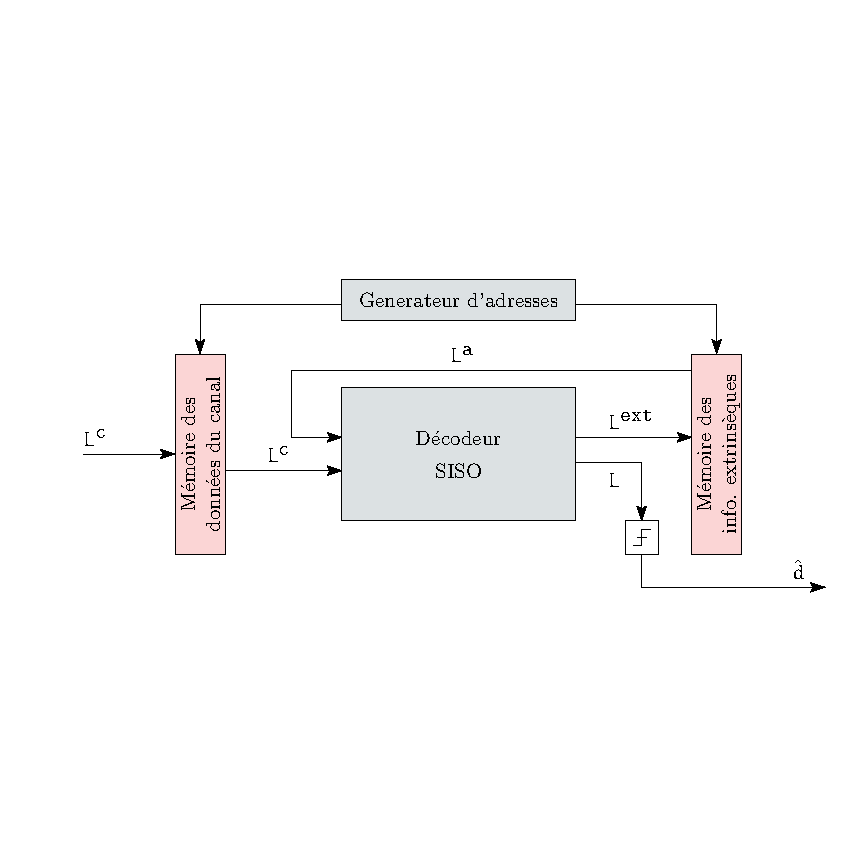
\includegraphics{main/ch4_fig/ipe/serial.pdf}
	\caption{Turbo décodage séquentiel. \label{fig:turbo_seq}}
\end{figure} 
 
\subsubsection{BCJR séquentiel}
Comme il a été présenté précédemment, l'algorithme choisi permettant l’obtention des informations \textit{a posteriori}
est l'algorithme MAP, ou plutôt une des ses simplifications comme l'algorithme EML-MAP. Cet algorithme repose sur trois
calculs successifs et séquentiels. Tous d'abord, le calcul des métriques de branches, notées $\gamma$, est réalisé. Ceci 
permet d’entamer le calcul récursif des métriques de nœuds aller, notées $\alpha$, combinant la transition du treillis 
courante ainsi que la section de treillis précédente. Le calcul récursif des métriques de nœuds retour, notées $\beta$, 
est similaire mais basé sur 
la section de treillis futur. Finalement, les information \textit{a posteriori} sont 
calculées en combinant ces trois métriques $\alpha$, $\beta$ et $\gamma$. 

Comme dans le cas de l'algorithme de Viterbi, chaque calcul de métrique de nœud est réalisé par un opération ACS 
(Addition-Comparaison-Sélection). En multipliant le
nombre d'unités ACS par le nombre de nœuds d'une section de treillis du code, il est possible de calculer toutes les
métriques de nœud aller ou retour d'une même section de treillis en même temps. Ce parallélisme ne nécessite que peu 
de surcoût puisque seulement les unités ACS sont dupliquées sans nécessiter de mémorisation supplémentaire car chaque 
opération d'ACS est exécutée sur le même jeu de données pour chacune des sections du treillis. Ainsi, l'ensemble des 
métriques de nœud d'une section de treillis peut être calculé en un coup d'horloge. Le calcul récursif des métriques de 
nœuds nécessite alors K cycles d'horloge.

Il est aussi possible d'effectuer en même temps le calcul de la métrique retour et celui de l'information \textit{a 
posteriori}. En effet, comme les métriques aller ont déjà été obtenues, dès que les métriques de nœud retour d'une 
section de treillis sont calculées, l'obtention de l'information \textit{a posteriori} ou extrinsèque est possible.
C'est ordonnancement des opérations correspond à celui originellement proposé par Bahl, Cocke, Jelinek et Raviv lors de 
la présentation de leur algorithme de décodage \cite{bcjr}. 
Finalement, sans considérer les bits de terminaison du treillis, qui ne sont 
jamais pris en compte dans ce chapitre afin d'exprimer plus simplement les nombre de cycles nécessaire, le temps requis 
pour exécuter une demi-itération du processus de décodage
itératif équivaut à $2\times K$ cycles d'horloge. La Figure \ref{fig:siso_seq} présente l'ordonnancement de ces
différentes opération dans ce contexte. Cet ordonnancement est appelé BCJR aller-retour.

\begin{figure}[!h]
	\centering
	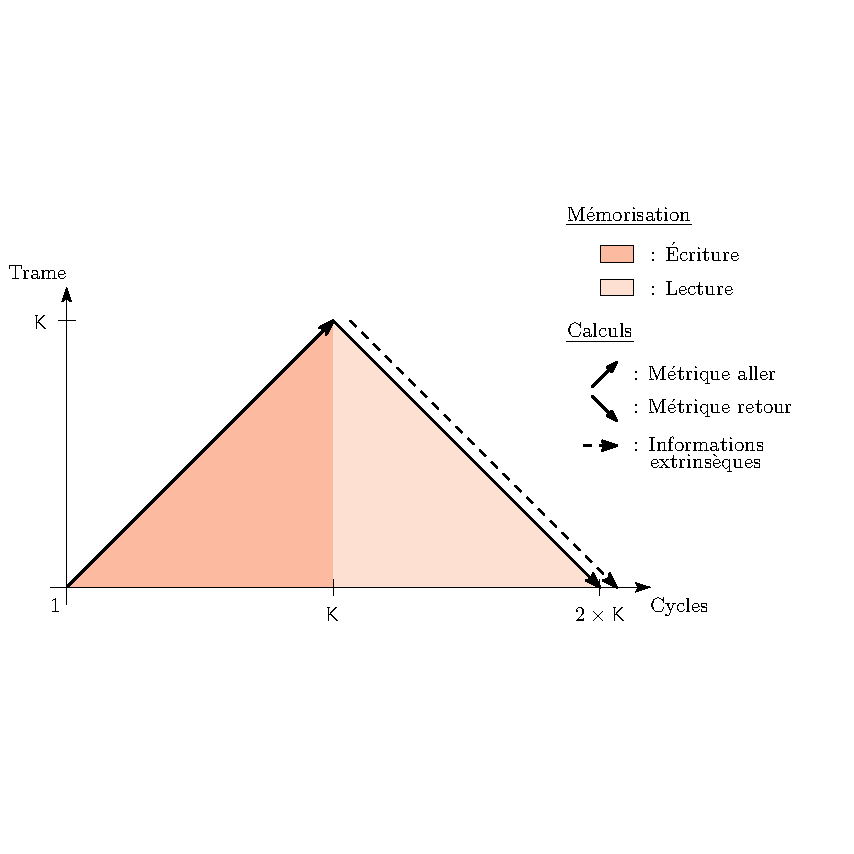
\includegraphics{main/ch4_fig/ipe/FB+LEG.pdf}
	\caption{BCJR Aller-Retour. \label{fig:siso_seq}}
\end{figure}

\subsubsection{BCJR parallèle}
Afin d'augmenter le niveau de parallélisme, il est possible de commencer le calcul des métriques de nœuds aller et des
métriques de nœuds retour en même temps. Dans ce cas, à partir de a moitié du parcours du treillis, deux informations 
extrinsèques sont produites en même temps. Cet ordonnancement est nommé BCJR butterfly \cite{butterfly} est est présenté 
en Figure \ref{fig:siso_but}. De la sorte, uniquement $K$ cycles d'horloge sont nécessaires pour effectuer une 
demi-itération de turbo décodage. L'effort de mémorisation reste inchangé par rapport au BCJR aller-retour. En revanche 
les informations extrinsèques sont produites par paires à partir du $K/2^{\text{ième}}$ cycle. Cette ordonnancement 
permet donc de réduire la latence du turbo décodage d'un facteur deux vis-à-vis de l'ordonnancement aller-retour.

\begin{figure}[!h]
	\centering
	\includegraphics{main/ch4_fig/ipe/BF_SW.pdf}
	\caption{BCJR Retour-Aller avec fenêtre glissante . \label{fig:siso_sw}}
\end{figure}

\begin{figure}[h]
	\centering
	\includegraphics{main/ch4_fig/ipe/BFLY.pdf}
	\caption{BCJR Butterfly. \label{fig:siso_but}}
\end{figure}

\begin{figure}[!h]
	\centering
	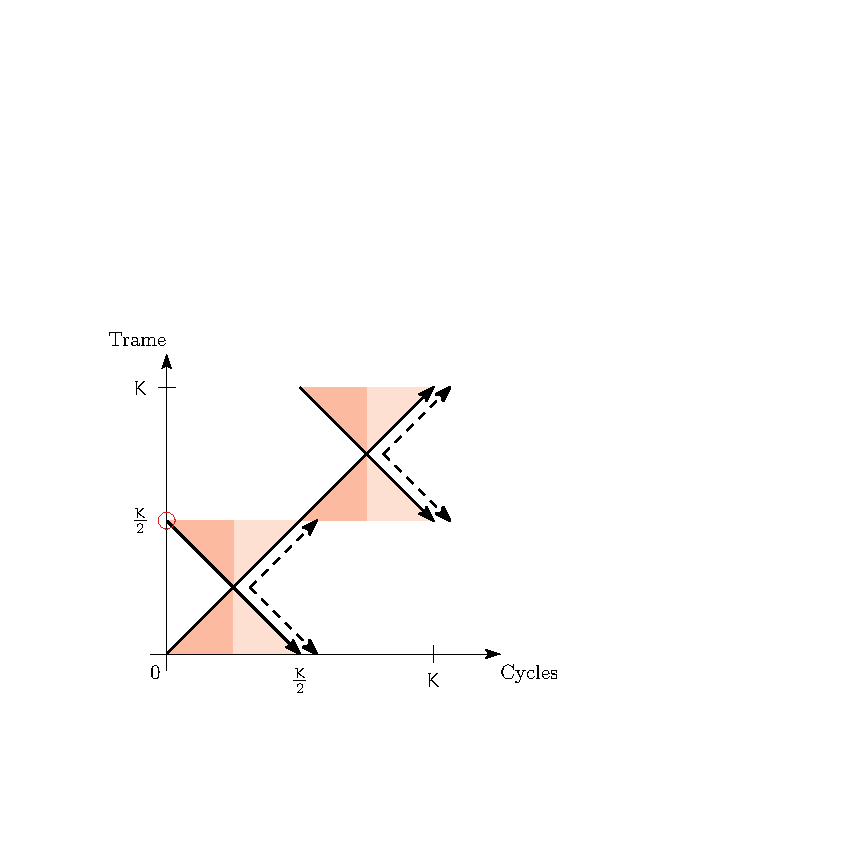
\includegraphics{main/ch4_fig/ipe/BFLY_SW.pdf}
	\caption{BCJR Butterfly avec fenêtre glissante. \label{fig:siso_bf_sw}}
\end{figure}

À partir de cet ordonnancement, la technique de fenêtre glissante (sliding window) a été proposée. L'objectif de cette 
approche consiste en la réduction de la mémorisation nécessaire. Afin de minimiser la diminution des performances 
de décodages induites par la suppression de la récursion aux limites des sous-trames, deux techniques peuvent être 
envisagées. La première est basée sur le calcul d'une fenêtre d'acquisition ou prologue. Dans ce cas, le calcul des 
métriques de nœud retour est commencé sur quelques sections de treillis suivant la limite de la taille du sous bloc. 
Une étude empirique a montré que la taille de ce prologue présentant le meilleur compromis entre calcul supplémentaires
et amélioration des performances de décodage est situé entre 3 et 5 fois la longueur de contrainte du code \cite{sw_init}.
La seconde technique est appelé passage de message. son principe consiste à utiliser les métriques de nœud calculées 
lors de l'itération précédente. Cette technique propose les meilleurs performances de décodage pour un surcoût de
mémorisation limité.

Le décodage par fenêtre glissante permet de considérer aisément un parallélisme au niveaux du décodage SISO. Ceci est 
abordé dans la prochaine section.

\subsection{SISOs en parallèle}
À partir de l'algorithme par fenêtre glissante, afin de gagner un niveau de parallélisme supplémentaire, il suffit 
d'augmenter le nombre de décodeurs SISO fonctionnant en même temps. Chacun opère alors sur un fenêtre de la trame 
différente, correspondant à une fenêtre de glissement. La Figure \ref{fig:sisos_par} présente ce type de parallélisme 
Pour $L=2$.

Ainsi, un second niveau de parallélisme peut être considéré en divisant la trame en sous-trame. Dans le cas d'un degré de 
parallélisme de 2, deux décodeurs SISO se répartissent sur la trame, l'un s'occupant des informations allant de l'index
1 à K/2, l'autre de K/2+1 à K. À nouveau, une initialisation aux limites des sous-trames est nécessaire. Les mêmes 
techniques que présentées précédemment peuvent être envisagées. Cependant, cette fois, en plus des métrique de nœuds
retour, les métriques de nœud aller doivent aussi être considérées. Aussi ce degré de parallélisme nécessite que 
l'entrelaceur puisse lui aussi être parallélisé afin qu’aucun conflit d'accès ne puisse apparaître 
\cite{interleaver_conflict}. 

\begin{figure}[!h]
	\centering
	\includegraphics{main/ch4_fig/ipe/BFLY_SB.pdf}
	\caption{SISO Butterfly en parallèle. \label{fig:sisos_par}}
\end{figure}

A nouveau le processus peut être 

\begin{figure}[!h]
	\centering
	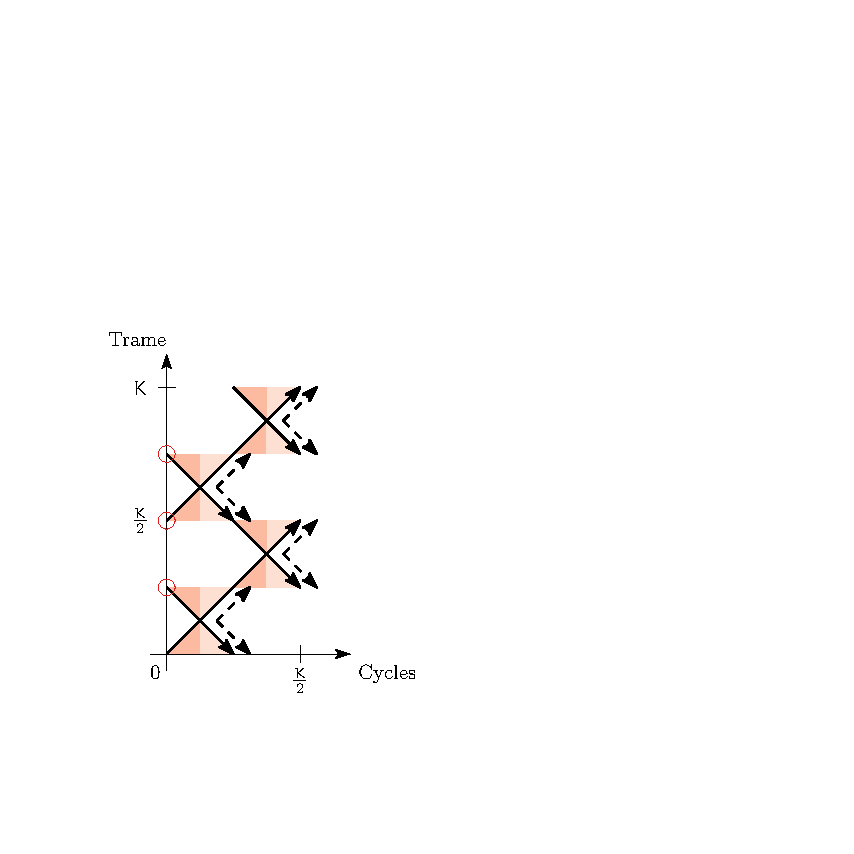
\includegraphics{main/ch4_fig/ipe/BFLY_SB_SW.pdf}
	\caption{SISO Butterfly avec fenêtre glissante en parallèle. \label{fig:sisos_par_sb}}
\end{figure}

\subsection{Processus itératif parallèle}
Il est possible de faire opérer le décodage de deux codes composant le turbo décodeur en même temps \cite{turbo_par}. 
Dans ce cas, après chaque itération, chaque décodeur élémentaire travaillant dans un certain domaine fourni ses 
informations extrinsèques au décodeur élémentaire utilisant les données du canal de l'autre dimension.

En 2005, le décodage shuffled a été proposé \cite{turbo_shuff}. Le principe est similaire à celui présenté à l'instant. 
Cependant, les informations extrinsèques sont échangées entre les deux domaines dès qu'elles ont été calculées. Chaque 
décodeur composant a donc accès plus vite aux information \textit{a priori} mises à jour. Ceci a alors pour effet
d'augmenter la vitesse de convergence et permet donc de réduire le nombre d'itérations. La Figure \ref{fig:turbo_shuff} 
présente l'échange d'informations extrinsèques au cours du processus de décodage shuffled avec deux décodeurs composants
travaillant en simultané.

\begin{figure}[!h]
	\centering
	\includegraphics{main/ch4_fig/ipe/shuffled.pdf}
	\caption{Turbo décodage Shuffled. \label{fig:turbo_suff}}
\end{figure}

Enfin la dernière méthode permettant de paralléliser le processus itératif de décodage revient à dupliquer l'ensemble 
du turbo décodeur afin de décoder différentes trames en même temps. Cette méthode revient à utiliser une architecture 
pipeline pour le décodeur. Dans ce cas, la profondeur maximale du pipeline équivaut à deux fois le nombre d'itération 
maximal permis. Bien que permettant une augmentation 
conséquente du débit, cette approche ne réduit pas la latence du processus de décodage alors qu'elle est couteuse sur 
le plan matériel puisque toutes les ressources calculatoires et de mémorisation sont dupliquées.


\section{Conclusion}
Récapitualtion:
Tableau 


\newpage
\section{Études de l'impact des paramètres de l'algorithme}
L'algorithme FNC est fonction de plusieurs paramètres ayant un impact à la fois sur les performances de décodage et sur
la complexité calculatoire. Cette section vise à présenter le meilleur compromis entre ces différents paramètres.

Le premier groupe de paramètres correspond au choix des itérations du processus de turbo décodage sur lesquelles le 
principe FNC est appliqué. Il a été présenté dans le chapitre précédent que si l'itération minimale à partir de laquelle


Première adaptation: passage sur les infos dans l'ordre naturel

Impact négatif d'un Imin trop faible.

Impact de la réduction de q sur les performances